\documentclass[aspectratio=169,11pt]{beamer}

\usepackage{fontspec}
\usepackage[ngerman]{babel}
\usepackage{graphicx}
\usepackage{microtype}
\usepackage{hyperref}
\usepackage{tikz}
\usetikzlibrary{positioning}

\setsansfont{Source Sans 3}
\setmonofont{Source Code Pro}

\definecolor{Tinte}{HTML}{1C2416}
\definecolor{Akzent}{HTML}{4D7027}
\definecolor{Akzent2}{HTML}{638044}
\definecolor{Papier}{HTML}{F5F7EF}
\definecolor{Flaeche}{HTML}{EAF1DF}
\definecolor{Sekundaer}{HTML}{53604B}
\definecolor{Linie}{HTML}{B7C99B}

\setbeamercolor{normal text}{fg=Tinte,bg=Papier}
\setbeamercolor{frametitle}{fg=Tinte,bg=Papier}
\setbeamercolor{block title}{fg=Akzent}
\setbeamercolor{structure}{fg=Akzent}
\setbeamercolor{alerted text}{fg=Akzent}
\setbeamercolor{itemize item}{fg=Akzent}
\setbeamercolor{itemize subitem}{fg=Akzent2}
\setbeamercolor{footline}{fg=Sekundaer,bg=Papier}
\setbeamerfont{frametitle}{size=\Large,series=\bfseries}
\setbeamertemplate{navigation symbols}{}
\setbeamertemplate{itemize item}{\raisebox{0.1ex}{\color{Akzent}\normalsize\textbullet}}
\setbeamertemplate{itemize subitem}{\raisebox{0.1ex}{\color{Akzent2}\small\textbullet}}
\setbeamertemplate{frametitle}{
  \vspace{0.2em}
  \insertframetitle\par
  {\small\color{Sekundaer}\insertframesubtitle}\par
  \vspace{0.2em}
  {\color{Akzent}\rule{0.08\linewidth}{1.5pt}}
}
\setbeamertemplate{footline}{
  \leavevmode
  \hbox to \paperwidth{
    \hspace{1.2em}\color{Sekundaer}\scriptsize Is it vegan? \hspace{0.6em} Web Engineering 1
    \hfill
    \color{Sekundaer}\scriptsize \insertframenumber/\inserttotalframenumber\hspace{1.2em}
  }
  \vskip 0.5em
}
\hypersetup{
  colorlinks=true,
  urlcolor=Akzent,
  linkcolor=Tinte
}

\title{Is it vegan?}
\author{Oliver Kühn}
\institute{Web Engineering 1 \textperiodcentered{} DHBW Karlsruhe}
\date{}

\begin{document}

\begin{frame}[plain]
  \vspace*{1.1cm}
  {\color{Akzent}\small\bfseries WEB ENGINEERING 1 \hspace{0.5em}/\hspace{0.5em} PROJEKTPRÄSENTATION}

  \vspace{0.75cm}
  {\Huge\bfseries Is it vegan?}

  \vspace{0.25cm}
  {\Large Ein Produkt-Check für den Einkauf -- von der EAN zur Einschätzung.}

  \vspace{1cm}
  {\color{Linie}\rule{\linewidth}{0.6pt}}

  \vspace{0.5cm}
  \begin{columns}[T,onlytextwidth]
    \column{0.55\textwidth}
      \small Oliver Kühn\\
      DHBW Karlsruhe
    \column{0.45\textwidth}
      \small\color{Sekundaer} Live-App\\
      \href{https://blccming.github.io/isitvegan/}{blccming.github.io/isitvegan}
  \end{columns}

\end{frame}

\begin{frame}{Was ich gebaut habe}
  \framesubtitle{Kurzüberblick}
  \begin{columns}[T,onlytextwidth]
    \column{0.55\textwidth}
      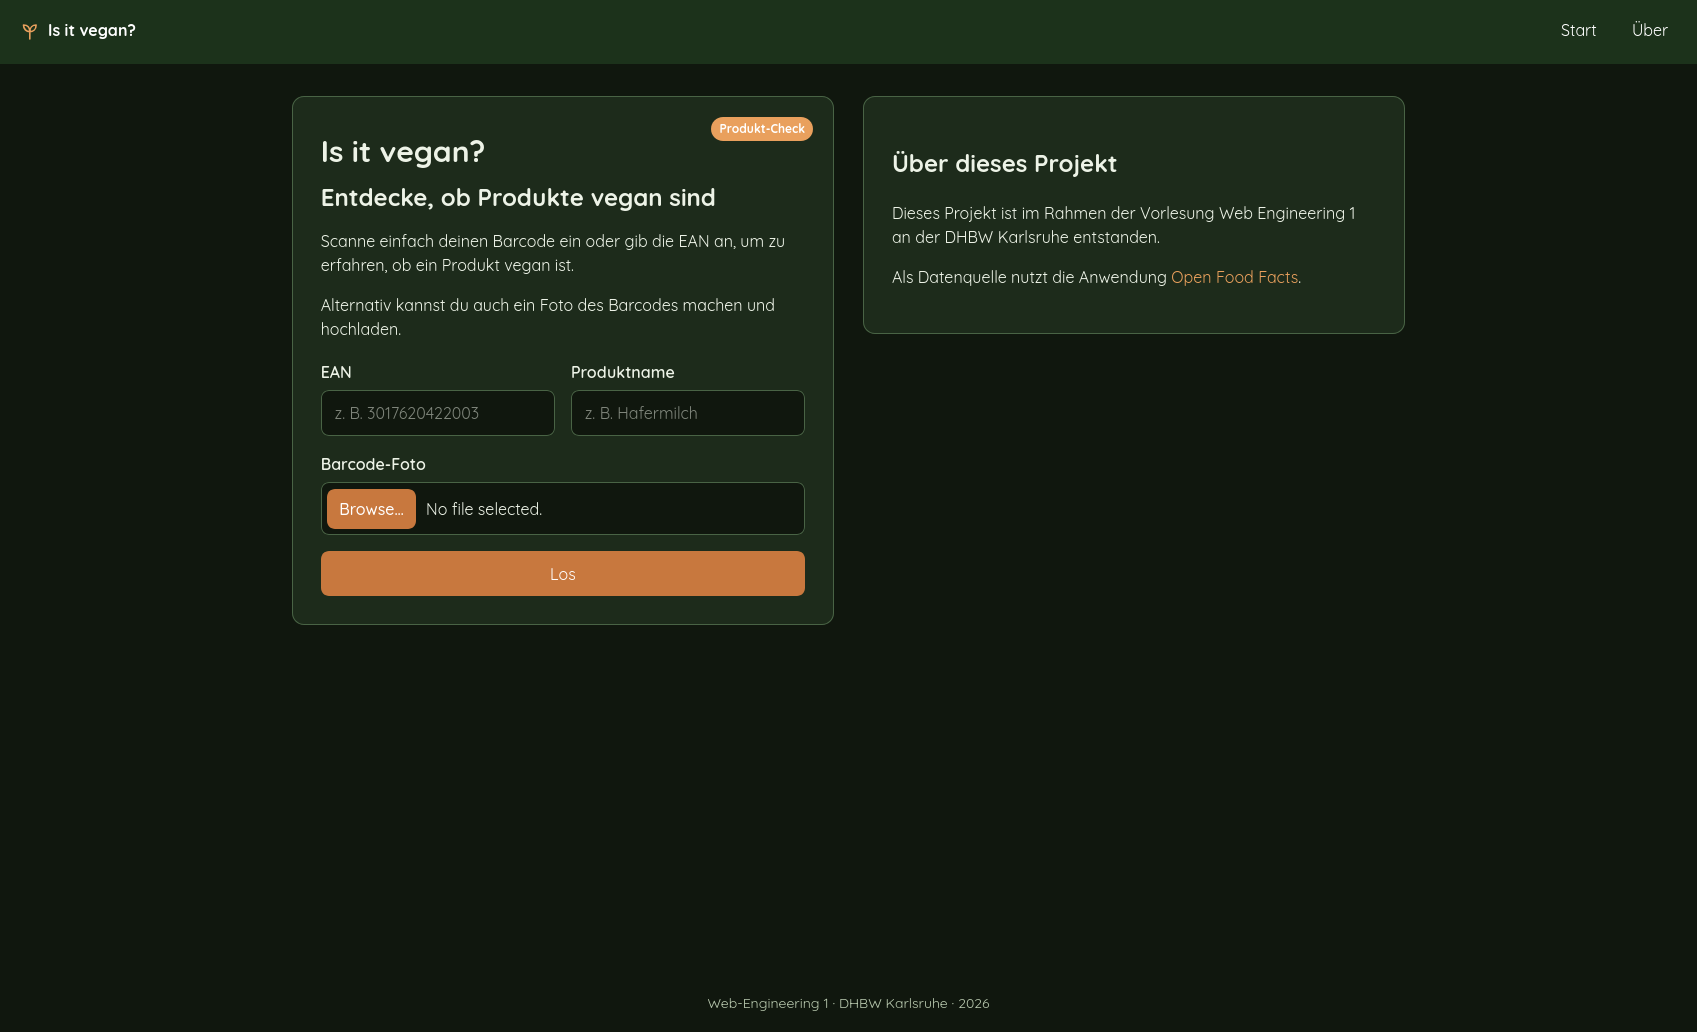
\includegraphics[width=\linewidth,height=0.62\textheight,keepaspectratio]{Screenshot.png}
    \column{0.4\textwidth}
      \vspace{0.15cm}
      {\large\bfseries Produkt-Check im Browser}

      \vspace{0.2cm}
      \small
      EAN und Produktname eingeben oder Barcode-Foto auswählen: Die App liest die Nummer und fragt Open Food Facts ab.

      \vspace{0.2cm}
      \begin{itemize}
        \item Status: vegan, nicht vegan oder unklar.
        \item Verlauf bleibt nach dem Neuladen erhalten.
        \item Bei Datenlücken: „Unklar“ statt raten.
      \end{itemize}
  \end{columns}
\end{frame}

\begin{frame}{Code und Architektur}
  \framesubtitle{Datenfluss, Zuständigkeiten und Entscheidungen}
  \centering
  \begin{tikzpicture}[
    box/.style={
      draw=Linie, fill=Flaeche, rounded corners=3pt, line width=0.8pt,
      text width=2.6cm, minimum height=1.05cm, align=center,
      inner sep=5pt, font=\small
    },
    pfeil/.style={draw=Akzent, line width=1.2pt, -stealth}
  ]
    \node[box] (manuell) at (0,0) {\textbf{Manuell}\\EAN eintippen};
    \node[box] (foto) at (0,-1.4) {\textbf{Foto-Scan}\\ZXing liest die EAN};
    \node[box] (daten) at (3.5,-0.7) {\textbf{Produktdaten}\\Cache oder Open Food Facts};
    \node[box] (ergebnis) at (6.8,-0.7) {\textbf{Ergebnis}\\Status und Verlauf};
    \draw[pfeil] (manuell.east) -- (daten.west);
    \draw[pfeil] (foto.east) -- (daten.west);
    \draw[pfeil] (daten) -- (ergebnis);
  \end{tikzpicture}

  \vspace{-0.2cm}
  \begin{columns}[T,onlytextwidth]
    \column{0.47\textwidth}
      {\large\bfseries Im Projekt}
      \small
      \begin{itemize}
        \item HTML/CSS: Oberfläche; \texttt{app.js}: Formular, API und Zustand.
        \item Vite \(\rightarrow\) \texttt{dist/} \(\rightarrow\) GitHub Actions \(\rightarrow\) Pages.
      \end{itemize}
    \column{0.47\textwidth}
      {\large\bfseries Bewusste Entscheidungen}
      \small
      \begin{itemize}
        \item Nur Tags \texttt{en:vegan}/\texttt{en:non-vegan} sind eindeutig, sonst „Unklar“.
        \item Verlauf in \texttt{localStorage}; API-Cache pro EAN. Öffentliche API direkt im Browser.
      \end{itemize}
  \end{columns}
\end{frame}

\begin{frame}{Vorgehen: vom Grundgerüst zum Live-Check}
  \framesubtitle{Sechs Ausbaustufen}
  \centering
  \begin{tikzpicture}[
    schritt/.style={
      draw=Linie, fill=Flaeche, rounded corners=4pt, line width=0.8pt,
      text width=3cm, minimum height=1.25cm, align=center,
      inner sep=7pt, font=\small
    },
    fluss/.style={draw=Akzent, line width=1.3pt, -stealth}
  ]
    \node[schritt] (start) at (0,0) {
      \textcolor{Akzent}{\textbf{30.09 \textperiodcentered{} Start}}\\
      HTML-Grundgerüst\\+ Vorlage
    };
    \node[schritt] (idee) at (4,0) {
      \textcolor{Akzent}{\textbf{14.10 \textperiodcentered{} Oberfläche}}\\
      Single-Page\\Formular + Layout\\SEO/Metadaten
    };
    \node[schritt] (stack) at (8,0) {
      \textcolor{Akzent}{\textbf{21.–27.10 \textperiodcentered{} Design}}\\
      Responsive Layout\\Tailwind + Pages
    };
    \node[schritt] (interaktion) at (8,-2.2) {
      \textcolor{Akzent}{\textbf{19.11 \textperiodcentered{} Interaktion}}\\
      Ergebnis + Verlauf\\localStorage + Sicherheits-Check
    };
    \node[schritt] (daten) at (4,-2.2) {
      \textcolor{Akzent}{\textbf{24.11 \textperiodcentered{} API + Scan}}\\
      Open Food Facts\\ZXing + Cache
    };
    \node[schritt] (live) at (0,-2.2) {
      \textcolor{Akzent}{\textbf{24.11 \textperiodcentered{} Live-Fix}}\\
      Pages-Pfad korrigiert\\Live-Version geprüft
    };
    \draw[fluss] (start) -- (idee);
    \draw[fluss] (idee) -- (stack);
    \draw[fluss] (stack.south) -- (interaktion.north);
    \draw[fluss] (interaktion.west) -- (daten.east);
    \draw[fluss] (daten.west) -- (live.east);
  \end{tikzpicture}
\end{frame}

\begin{frame}{KI im Projekt}
  \framesubtitle{Werkzeuge, Einsatz und eigene Prüfung}
  \begin{columns}[T,onlytextwidth]
    \column{0.47\textwidth}
      {\large\bfseries Wo KI geholfen hat}
      \small
      \begin{itemize}
        \item Copilot half bei Ideen, Tailwind-Umsetzung, API/ZXing und Deployment.
        \item Claude Code unterstützte Formular ohne Reload, Zustandsobjekt und gefilterten Verlauf.
        \item Beispielprompt: \glqq Generiere mir 5 Projektideen für eine Webapp, die den Alltag erleichtern.\grqq{}
      \end{itemize}
    \column{0.47\textwidth}
      {\large\bfseries Was ich selbst prüfen musste}
      \small
      \begin{itemize}
        \item Ein erster Verlaufsentwurf nutzte eigenes CSS statt des Tailwind-Ansatzes im Projekt.
        \item Ich habe die Umsetzung angepasst und mit API-Antworten sowie der Live-Seite abgeglichen.
        \item KI lieferte Vorschläge und beschleunigte Umsetzung; Entscheidungen und Ergebnis blieben bei mir.
      \end{itemize}
  \end{columns}
\end{frame}

\begin{frame}{Was ich mitnehme}
  \framesubtitle{Erkenntnisse und nächster Schritt}
  \begin{columns}[T,onlytextwidth]
    \column{0.47\textwidth}
      {\large\bfseries Gelernt}
      \begin{itemize}
        \item Eine API kann Daten liefern, aber keine verlässliche Aussage: fehlende Analyse-Tags bedeuten „Unklar“.
        \item EAN-Eingabe, Foto-Scan, API-Fehler und Deployment sind Teil derselben Nutzerreise.
        \item Browser-Speicher braucht Datenprüfung und Versionswechsel, nicht nur ein \texttt{setItem}.
      \end{itemize}
    \column{0.47\textwidth}
      {\large\bfseries Beim nächsten Projekt}
      \begin{itemize}
        \item API-Antworten und Grenzfälle von Anfang an als Testfälle festhalten.
        \item Foto-Scan früher auf echten Mobilgeräten ausprobieren.
        \item Zuständigkeiten für Oberfläche, Datenzugriff und Speicherung früher trennen.
      \end{itemize}
  \end{columns}
\end{frame}

\begin{frame}[plain]
  \vspace*{1.1cm}
  {\color{Akzent}\small\bfseries RÜCKFRAGEN}

  \vspace{0.5cm}
  {\Huge\bfseries Danke.}

  \vspace{0.3cm}
  {\Large Was möchtet ihr wissen?}

  \vspace{1cm}
  {\color{Linie}\rule{\linewidth}{0.6pt}}

  \vspace{0.5cm}
  \small
  Live-App: \href{https://blccming.github.io/isitvegan/}{blccming.github.io/isitvegan}\\
  Code und Commit-Historie: \href{https://github.com/blccming/isitvegan}{github.com/blccming/isitvegan}
\end{frame}

\end{document}
